\chapter{AdaptaMaterialEscolar 2.0}
\label{cap:AdaptaMaterialEscolar2.0}
En este capítulo explicaremos la obtención de requisitos y su priorización en la Sección \ref{cap:requisitos}. También se describirá la iteración competitiva para el diseño de la aplicación en la Sección \ref{disenyoDeLaAplicacion}.

\section{Requisitos}
\label{cap:requisitos}
En esta sección se explicara la tabla de requisitos.

Lo primero que realizamos fue analizar la memoria anterior extrayendo las funcionalidades que faltan por implementar y las propuestas por los profesores. Hemos agrupado estas funcionalidades en tres grupos: formato, ejericios y auxiliar. Quedando las funcionalidades agrupadas de la siguiente manera:
Formato: 
\begin{itemize}
  \item Añadir encabezado al texto.
  \item Añadir un tipo de fuente escolar.
  \item Añadir una leyenda de colores con la categoría de cada tipo.
  \item Añadir leyenda de colores para el tema de cada asignatura.
  \item Añadir ejercicios de matemáticas con cuadrícula para escribir los números.
  \item Añadir la alternativa de añadir doble pauta, en vez de renglones de una única línea, para determinar el tamaño de la letra del alumno.
  \item Crear tablas que organicen el temario y/o las actividades, seleccionando contenido.
  \item Crear esquemas que faciliten la visualización.
  \item Estandarizar formato para títulos e índices del temario.
  \item Enumerar ejercicios de forma automática.
\end{itemize}
Ejercicios:
\begin{itemize}
  \item Ejercicios de relacionar contenido mediante flechas.
  \item Añadir ejercicios de cálculo con huecos a rellenar por el alumno.
  \item Añadir ejercicios con espacio para dibujar.
  \item Ejercicios de completar los espacios en blanco en tablas y esquemas.
\end{itemize}
Auxiliar:
\begin{itemize}
  \item Generar un resumen a partir de un texto.
  \item Exportar el documento a formato Word para hacer modificaciones.
  \item Añadir un pictotraductor como funcionalidad.
  \item Añadir imágenes buscando una palabra en bases de datos de imágenes libres
  \item Sustituir una palabra por una imagen.
  \item Crear una herramienta de recorte de imágenes para el texto original.
\end{itemize}
Tras haber analizado en detalle las  funcionalidades anteriores hemos encontrado que varias funciones ya están realizadas y otras no se van a implementar por falta de información.
Funciones realizadas:
\begin{itemize}
  \item Añadir encabezado al texto.
  \item Enumerar ejercicios de forma automática.
\end{itemize}
Funciones sin información suficiente:
\begin{itemize}
  \item Añadir imágenes buscando una palabra en bases de datos de imágenes libres
  \item Sustituir una palabra por una imagen.
  \item Crear una herramienta de recorte de imágenes para el texto original.
  \item Crear tablas que organicen el temario y/o las actividades, seleccionando contenido.
  \item Crear esquemas que faciliten la visualización.
  \item Ejercicios de completar los espacios en blanco en tablas y esquemas.
\end{itemize}
Por lo tanto las fuciones a implementar son las que se muestran en la tabla \ref{Funciones}.
\begin{table}[]
  \begin{tabular}{|l|l|l|l|}
  \hline
  Funciones                                                                                                                                                                            & Coste & Importancia & Prioridad \\ \hline
  Generar un resumen a partir de un texto.                                                                                                                                             & 5     & 5           & 25        \\ \hline
  \begin{tabular}[c]{@{}l@{}}Exportar el documento a formato Word para \\ hacer modificaciones.\end{tabular}                                                                           & 5     & 5           & 25        \\ \hline
  Añadir un pictotraductor como funcionalidad.                                                                                                                                         & 5     & 4           & 20        \\ \hline
  \begin{tabular}[c]{@{}l@{}}Ejercicios de relacionar contenido mediante \\ flechas.\end{tabular}                                                                                      & 5     & 3           & 15        \\ \hline
  Añadir un tipo de fuente escolar.                                                                                                                                                    & 5     & 2           & 10        \\ \hline
  \begin{tabular}[c]{@{}l@{}}Añadir una leyenda de colores con la categoría \\ de cada tipo.\end{tabular}                                                                              & 4     & 2           & 8         \\ \hline
  \begin{tabular}[c]{@{}l@{}}Añadir ejercicios para ejercicios de cálculo con \\ fórmulas con huecos arellenar por el alumno.\end{tabular}                                             & 4     & 2           & 8         \\ \hline
  Añadir ejercicios con espacio para dibujar.                                                                                                                                          & 5     & 1           & 5         \\ \hline
  \begin{tabular}[c]{@{}l@{}}Añadir leyenda de colores para el tema de cada \\ asignatura(color borde personalizar colores).\end{tabular}                                              & 4     & 1           & 4         \\ \hline
  \begin{tabular}[c]{@{}l@{}}Añadir ejercicios de matemáticas con cuadrícula \\ para escribir los números.\end{tabular}                                                                & 3     & 1           & 3         \\ \hline
  \begin{tabular}[c]{@{}l@{}}Añadir la alternativa de añadir doble pauta, en vez \\ de renglones de una única línea, para determinar el \\ tamaño de la letra del alumno.\end{tabular} & 3     & 1           & 3         \\ \hline
  \begin{tabular}[c]{@{}l@{}}Estandarizar formato para títulos e índices del \\ temario.\end{tabular}                                                                                  & 1     & 1           & 1         \\ \hline
  \end{tabular}
  \caption{Funciones a implementar}
  \label{Funciones}
  \end{table}

\section{Diseño de la apliación}
\label{disenyoDeLaAplicacion}
Para el diseño de la aplicación web hemos realizado una iteración competitiva. Cada integrante del grupo ha proporcionado un diseño de la apliación como se muestra en las figuras \ref{IteracionCompetitiva1}, \ref{IteracionCompetitiva2}, \ref{IteracionCompetitiva3} y \ref{IteracionCompetitiva4}.
Una vez que cada integrante ha explicado su diseño, hemos cogido lo mejor de cada uno quedando la aplicación de la siguiente manera \ref{diseño_final}.


\begin{figure}[ht!]
    \centering
    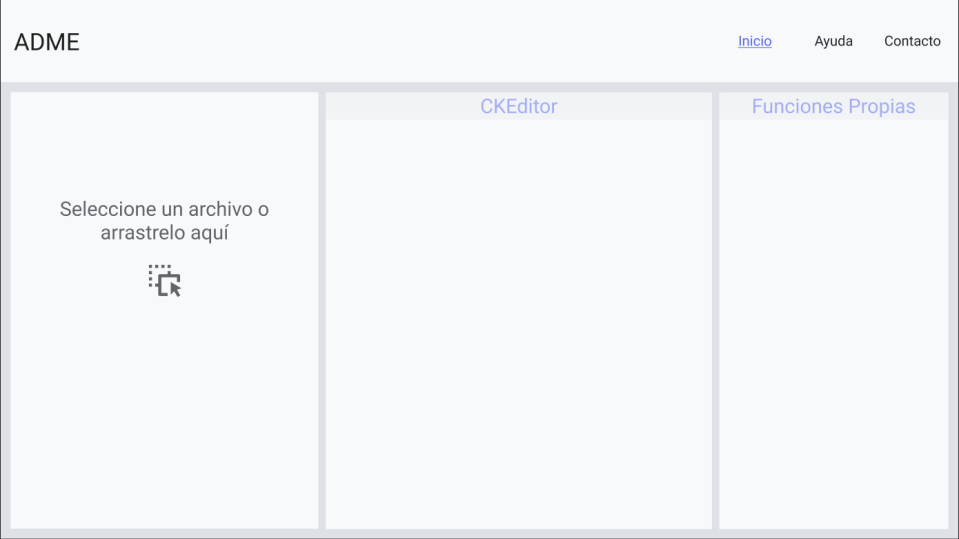
\includegraphics[scale=0.3]{Diseño/IteracionCompetitiva1}
    \caption{Diseño aplicación iteración competitiva 1.}
    \label{IteracionCompetitiva1}
\end{figure}
\begin{figure}[ht!]
    \centering
    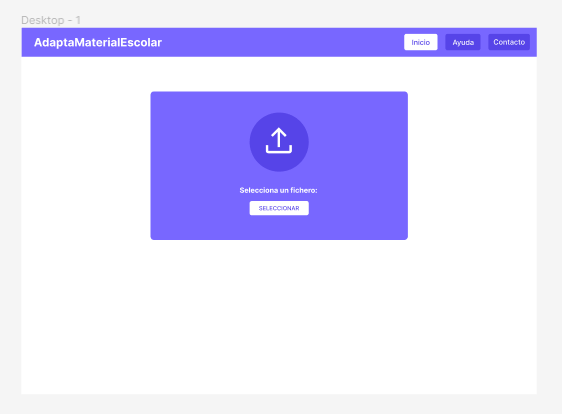
\includegraphics[scale=0.5]{Diseño/IteracionCompetitiva2}
    \caption{Diseño aplicación iteración competitiva 2.}
    \label{IteracionCompetitiva2}
\end{figure}
\begin{figure}[ht!]
    \centering
    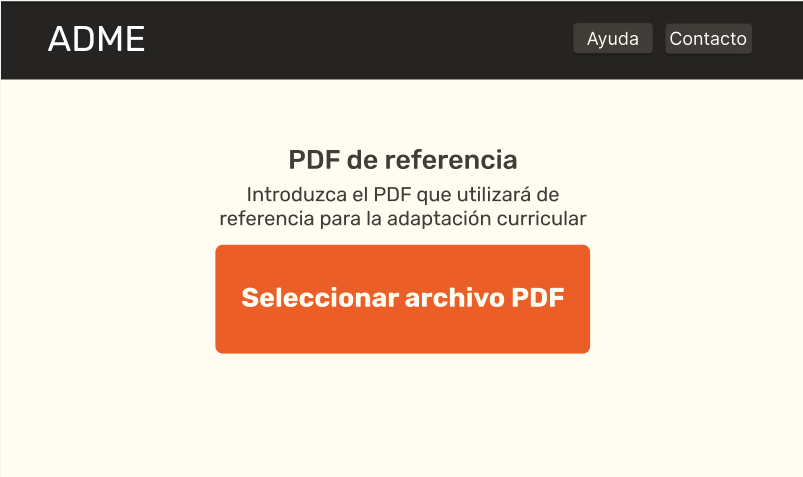
\includegraphics[scale=0.5]{Diseño/IteracionCompetitiva3}
    \caption{Diseño aplicación iteración competitiva 3.}
    \label{IteracionCompetitiva3}
\end{figure}
\begin{figure}[ht!]
    \centering
    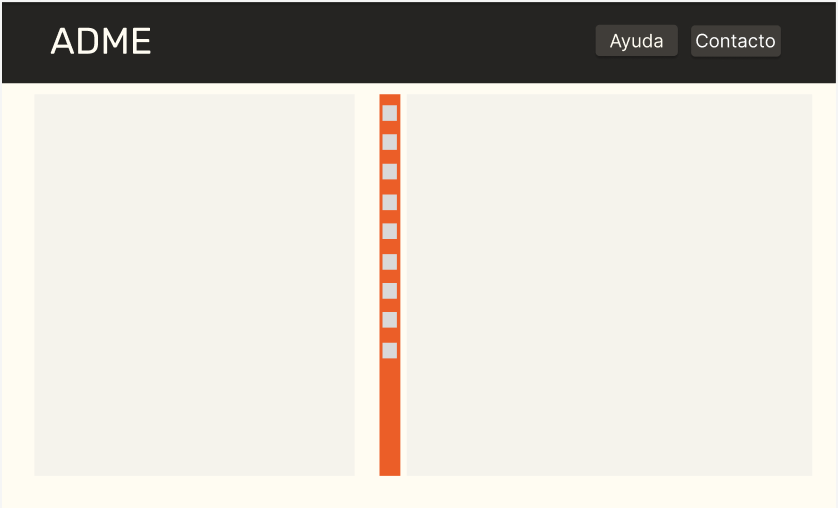
\includegraphics[scale=0.5]{Diseño/IteracionCompetitiva4}
    \caption{Diseño aplicación iteración competitiva 4.}
    \label{IteracionCompetitiva4}
\end{figure}
\begin{figure}[ht!]
  \centering
  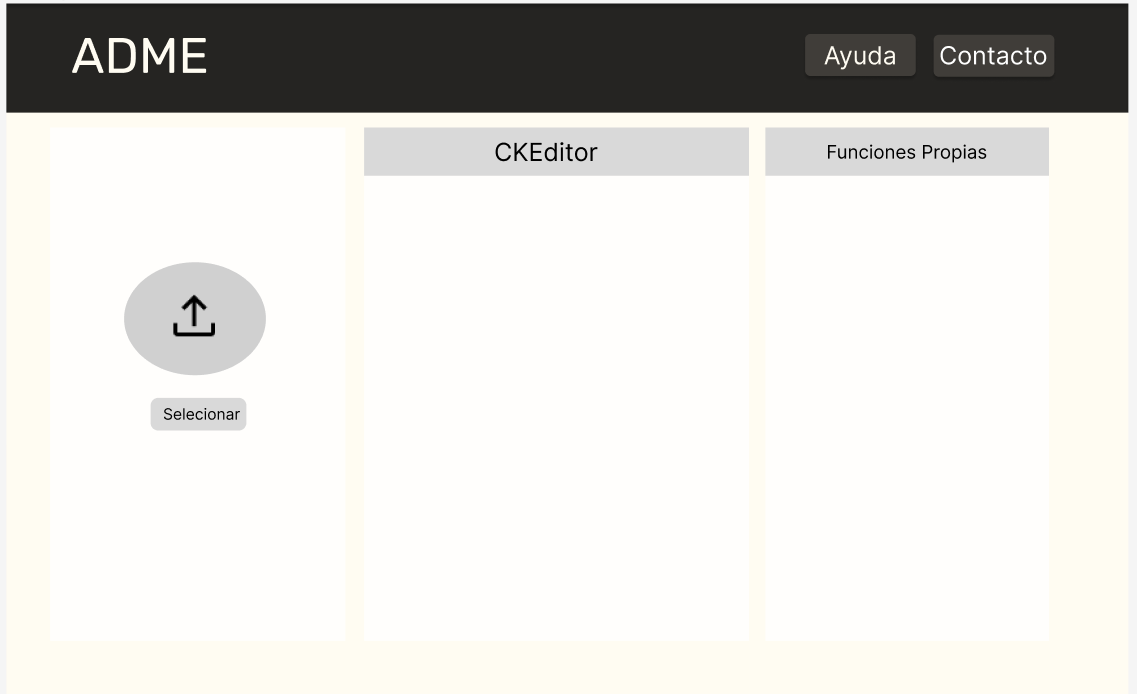
\includegraphics[scale=0.3]{Diseño/Diseño Final}
  \caption{Diseño final aplicación.}
  \label{diseño_final}
\end{figure}
